\begin{center}
    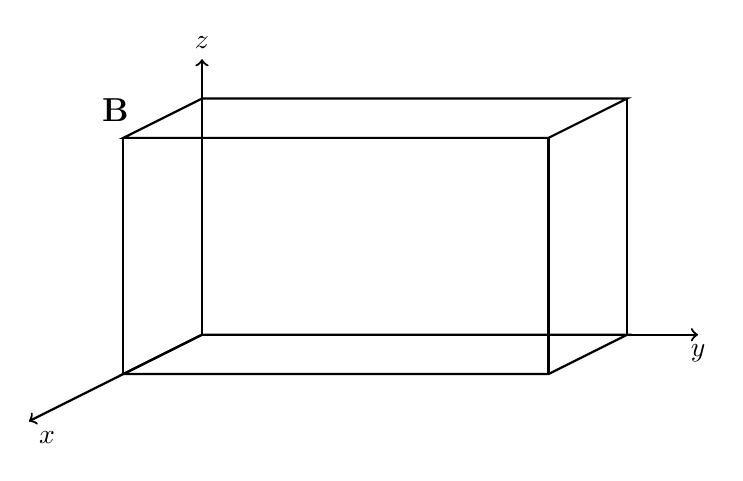
\begin{tikzpicture}[x={(0.9cm,0cm)}, y={(-1cm,-0.5cm)}, z={(0cm,1cm)}, scale=1]
    	
        % Paralelepípedo
        \draw[thick] (0,0,0) -- (6,0,0) -- (6,1,0) -- (0,1,0) -- cycle; % base
        \draw[thick] (0,0,3) -- (6,0,3) -- (6,1,3) -- (0,1,3) -- cycle; % parte superior
        \draw[thick] (0,0,0) -- (0,0,3);
        \draw[thick] (6,0,0) -- (6,0,3);
        \draw[thick] (6,1,0) -- (6,1,3);
        \draw[thick] (0,1,0) -- (0,1,3);
        
        % Ejes coordenados (x más largo que el paralelepípedo)
        \draw[->, thick] (0,0,0) -- (7,0,0) node[below] {\(y\)};
        \draw[->, thick] (0,0,0) -- (0,2.2,0) node[below right] {\(x\)};
        \draw[->, thick] (0,0,0) -- (0,0,3.5) node[above] {\(z\)};
        
        % Etiqueta B
        \node at (0,1.1,3.4) {\large \(\mathbf{B}\)};
        
    \end{tikzpicture}
\end{center}